\begin{frame}[c]{}
\begin{center}
    \textbf{Part II: Fixed Parameter (\textcolor{red}{In})Tractibility \& $w$-Hardness}
    
    \textit{Stepping towards lower-bounds for FPT}
    
\end{center}
\end{frame}

\begin{frame}[c]{Parametrized Hardness}

\pause\textbf{By Now: } Denote $\omega[1]$ as problems that might not expose a FPT algorithm. 

\pause\textbf{Goal:} A theory of Intractibility for Parametrized Problems
\begin{center}
    \begin{table}[]
    \begin{tabular}{@{}lll@{}}
     \topline
     & \textbf{NP-Hardness} & \textbf{W[1]-Hardness} \\
     \midrule
     \pause\textbf{Objects of Study} & "Classical" $L\subseteq \{0,1\}^*$ & "Parametrized" $L\subseteq \{0,1\}^* \times \mathbb{N}$  \\
     \pause\textbf{Tractibility} & PTIME & FPT \\
     \pause\textbf{Hardness Assumption} & $\texttt{SAT} \notin \texttt{PTIME} $ & $ \texttt{CLIQUE}_k \notin \texttt{FPT} $ \\
     \pause\textbf{Reductions} & Poly-Time Karb Reductions & {\color{green}{FPT Reductions}}  \\ \bottomrule
    \end{tabular}
\end{table}
\end{center}
\end{frame}


\begin{frame}[c]{Parametrized Reductions}
\begin{block}{Definition 4: Parametrized Reduction (\cite[Def 13.1]{Cygan2015})}
Let $A,B\subseteq \Sigma^*\times\mathbb{N}$ two parametrized problems. A \textit{Parametrized Reduction} from A to B is an algorithm that, given an instance $(x,k)$ of A, outputs an instance $(x', k')$ of B such that
\begin{itemize}
    \item $(x,k)$ is a \textcolor{gray}{yes instance} of A \textbf{iff} $(x',k')$ is a \textcolor{gray}{yes instance} of B \\
    \item $k' \leq g(k)$ for some computable function $g$
    \item the running time is $f(k)\cdot |x|^{\mathcal{O}(1)}$
\end{itemize}
\end{block}

\end{frame}

\begin{frame}[c]{Parametrized Reductions}
\begin{center}
\begin{block}{Theorem 1: Central Property of Parametrized Reductions (\cite[Th. 13.2]{Cygan2015})}{If there is a Parametrized Reduction from L to Q and Q is FPT, then L is FPT as well. }
\end{block}
\end{center}
\textbf{Proof: Follows from definition} 
\begin{itemize}
    \pause\item Suppose Q can be solved in $\mathtt{FPT\-TIME}$~ $f(l) \cdot |y|^c$ ) and the reduction $L \leq_{\mathtt{FPT}} Q$ takes time $g(k) \cdot |x|^d$
    \pause\item Then L solves in $f(h(k)) \cdot (g(k) \cdot |x|^d)^c$ as  l bounded by $l \leq h(k)$ (Property II) and the instance can not be larger then the duration of the reduction
    \item The final runtime only exponential in k and polynomial in |x| and hence FPT \QEDA
    \end{itemize}
\end{frame}

\begin{frame}[c]{Parametrized Reductions}
\begin{center}
\begin{block}{Theorem 2: Transitivity \cite[Th. 13.3]{Cygan2015}}
If there are Parametrized Reductions from  L to Q and from Q to T, then there is a Parametrized Reduction from L to T.
\end{block}
    \textbf{Proof: Omitted. Again directly from the Definition}
\end{center}
\end{frame}

\begin{frame}[c]{Towards a New Hierarchy}
\begin{center}
\begin{block}{(Rather Informal) Definition: The class $\omega[1]$}
$\omega[1] := [\mathtt{CLIQUE}_k]^{\mathtt{FPT}}$ (All problems FPT-reducible to $\mathtt{CLIQUE}_k$)
\end{block}
\begin{itemize}
    \pause\item Problem Q is $\omega[1]$-hard iff $\mathtt{CLIQUE}_k$ reduces to it.
    \pause\item $\mathtt{FPT} \subseteq \omega[1]$
    \pause\item $P = NP \Rightarrow \mathtt{FPT} = \omega[1]$
    \pause\item If $\omega[1]$-hard problem is \mathtt{FPT} then also collapse $\mathtt{FPT} =  \omega[1]$
\end{itemize}
\end{center}
\end{frame}

\begin{frame}[c]{Recap: Independent Set}
\begin{center}
\begin{tcolorbox}[colback=green!5,colframe=green!40!black,title=$\mathtt{INDEPENDENT~SET}$ (See \cite{Cygan2015})]
\begin{columns}[T] % align columns
    \begin{column}{.18\textwidth}
    \\~
    
    \textbf{Input:}\\
    \textbf{Question:}
    \end{column}
    \begin{column}{.78\textwidth}
    \\~
    
    Graph G and integer k\\
    Does G has an independent set of size k?
    \\~
    
   \textit{In other words: Is there a vertex-set $S$ of size $k$  that are non-adjacent?}
    \end{column}
 \end{columns}
\end{tcolorbox}

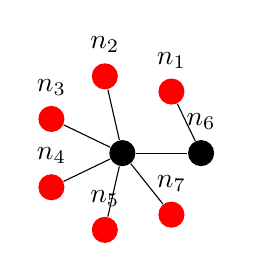
\begin{tikzpicture}
      \node[circle,fill=black] at (360:0mm) (center) {};
    \foreach \n in {2,...,5}{
        \node[circle,fill=red,label=$n_\n$] at ({\n*360/7}:1cm) (n\n) {};
        \draw (center)--(n\n);
    }
        \node[circle,fill=red,label={$n_1$}] at ({360/7}:1cm) (n1) {};
        \node[circle,fill=red,label={$n_7$}] at ({6*360/7}:1cm) (n6) {};
        \draw (center)--(n6);
        \node[circle,fill=black,label={$n_6$}] at ({7*360/7}:1cm) (n7) {};
        \draw (n1) -- (n7);
        \draw (center)--(n7);
\end{tikzpicture}
\end{center}
\end{frame}

\begin{frame}[c]{A First Trivial Reduction: $\mathtt{CLIQUE}_k \leq_{\mathtt{FPT}} \mathtt{IS}_k$}
\begin{center}

\begin{itemize}
    \pause\item It is known: Graph G has $\mathtt{IS}$ of size k if and only if $G^{-1}$ has a $\mathtt{CLIQUE}$ of size k.
    \pause\item Therefore: $(G, k) \longrightarrow (G^{-1}, k)$ directly gives the desired reduction (Even in PTIME!).
\end{itemize}
\end{center}
\end{frame}

\begin{frame}[c]{Why Standard Reductions Not Always Work:  $\mathtt{VC}_k \leq_{\mathtt{FPT??}} \mathtt{IS}_k$}
\begin{center}

\begin{itemize}
    \pause\item Again, it is known: X is a $\mathtt{VC}$ if and only if $G - X $ is an $\mathtt{IS}$.
    \pause\item Therefore: $(G, k) \longrightarrow (G, n - k)$ gives indeed a reduction,  \textbf{but} %TODO Really? 
    \pause\item The parameter k is not bounded any more just by k!
\end{itemize}
\end{center}
\end{frame}



\begin{frame}[c]{Multicolored Clique}
\begin{center}
\begin{tcolorbox}[colback=green!5,colframe=green!40!black,title=\textrm{MULTICOLORED~CLIQUE~(PARTITIONED~CLIQUE) \cite[p. 428]{Cygan2015}}]
\begin{columns}[T] % align columns
    \begin{column}{.18\textwidth}
    \\~
    
    \textbf{Input:}\\
    \textbf{Question:}
    \end{column}
    \begin{column}{.78\textwidth}
    \\~
    
    Graph G, integer k, partition $(V_1, ...V_k)$\\
    Does G has a $k$-Clique containing \textbf{exactly} one vertex from each set $V_i$?
    \end{column}
 \end{columns}
\end{tcolorbox}
\end{center}
\end{frame}

\begin{frame}[c]{$\mathtt{CLIQUE}_k \leq_{\mathtt{FPT}} \mathtt{MULTICOLORED~CLIQUE}_k$}
\textbf{Idea: } Distribute a Clique to k partitions
    \begin{center}
        \includegraphics[scale=0.17]{img/Unbenannt.png}
    \end{center}
\textbf{Proof} 
\begin{itemize}
    \item $\mathtt{CLIQUE}_k \Rightarrow \mathtt{M\-CLIQUE}_k$: Distribute original clique to partitions
    \item $\mathtt{M\-CLIQUE} \Rightarrow \mathtt{CLIQUE}_k$: Project them back to a set of vertices of G
\end{itemize}
\textbf{Therefore: }$(G,k) \longrightarrow (G',k')$ is a FPT reduction. 
\end{frame}

\begin{frame}[c]{Notes}
\begin{itemize}
\item  For proofing $\omega[1]$ hardness, it is often useful to start with a $\mathtt{MULTICOLORED~CLIQUE}$
\item Similar, there is a FPT reduction from $\mathtt{INDEPENDENT~SET} \leq_{\mathtt{FPT}} \mathtt{MULTICOLORED~INDEPENDENT~SET}$
\end{itemize}
\end{frame}


\begin{frame}[c]{Dominating Set}

\begin{center}
\begin{tcolorbox}[colback=green!5,colframe=green!40!black,title=$\mathtt{DOMINATING~SET}$ (\cite{Cygan2015})]
\begin{columns}[T] % align columns
    \begin{column}{.18\textwidth}
    \\~
    
    \textbf{Input:}\\
    \textbf{Question:}
    \end{column}
    \begin{column}{.78\textwidth}
    \\~
    
    Graph G and Integer k\\
    Is there $X$ of size $k$ s.t. $N[X] = V(G)$?
    
    \end{column}
 \end{columns}
 
\\~

Where we denote $N[X]$ as the \textbf{close neighborhood} of $X$
\end{tcolorbox}
\end{center}

\textbf{Corollary: } $\mathtt{DOMINATING~SET}$ is $\omega[1]$-hard and $\omega[2]$-complete  

\end{frame}

\begin{frame}{Intuition About Differences of $\omega[1]$ and $\omega[2]$}

Formulating $\mathtt{CLIQUE}$ and $\mathtt{DOMINATING~SET}$ in logical terms \footnote{More precisely: Monadic Second-Order-Logic of Graphs}

\begin{center}
\begin{itemize}
    \item X is a $\mathtt{CLIQUE}$ iff $$\forall_{\mathrm{(u,v) \notin G}}: u \notin X \lor v \notin X $$
%    (Every non-edge, not both are in the Clique
    \item X is a $\mathtt{DOMINATING~SET}$ iff $$\forall u \exists v: v \in X \land (u,v) \in E(G) $$
\end{itemize}
\end{center}

\textbf{Recall: } The Polynomial Hierarchy also defined via quantifiers. 

\textbf{Maybe something similiar applies also in the FPT case?}

\end{frame}

\begin{frame}{Intuition About Differences of $\omega[1]$ and $\omega[2]$}
\begin{columns}[T] % align columns
    \begin{column}{.5\textwidth}
    sdsf
    \end{column}
    \begin{column}{.5\textwidth}
    lkj
    \end{column}
\end{columns}

  \begin{tikzpicture}[level/.style={sibling distance=15mm/#1}, scale = 0.8]
    \node [circle,draw] (z){$\land$}
    child {node [circle,draw] (a) {$\neg\land$}
        child {node [] (b) {$x_1$}
        }
  }
  child {node [circle,draw] (j) {$\neg \land$}
        child {node [] (c) {$x_2$}
        }
}
  child {node [circle,draw] (w) {$\neg \land$}
        child {node [] (d) {$x_3$}
        }
  }
  child {node [circle,draw] (q) {$\neg \land$}
        child {node [] (e) {$x_4$}
        }
  }
  child {node [circle,draw] (r) {$\neg \land$}
        child {node [] (f) {$x_5$}
        }
  }
  \draw (b) -- (c)
  
  \end{tikzpicture}
\end{frame}

\begin{frame}{Quick Outlook: Weighted Circuit Satisfiability}

\begin{tcolorbox}[colback=green!5,colframe=green!40!black,title=$\mathtt{WEIGHTED~CIRCUIT~SATISFIABILITY (WCS)}$ (\cite{Cygan2015})]
\begin{columns}[T] % align columns
    \begin{column}{.18\textwidth}
    \\~
    
    \textbf{Input:}\\
    \textbf{Question:}
    \end{column}
    \begin{column}{.78\textwidth}
    \\~
    
    Circuit C and Integer k\\
    
    Is there a satisfying valuation of the input \textbf{with exactly k ones}?
    
    \end{column}
 \end{columns}

\end{tcolorbox}


\textbf{Definition: } $\omega[t] := $ Problems FPT-Reducible to $\mathtt{WCS}$ for circuits of 
\begin{itemize}
    \item Constant Depth and
    \item weft at most t
\end{itemize}

\end{frame}


%TODO:: 
%https://wuecampus2.uni-wuerzburg.de/moodle/pluginfile.php/1564087/mod_resource/content/3/vl09-part2-printerversion.pdf
\begin{frame}[c]{Summary FPT Reductions\footnote{(Comp. \cite{fptland})}}
    \begin{center}
        \includegraphics[scale=0.3]{img/landscape.png}
    \end{center}
\end{frame}

\begin{frame}[c]{Key Takeaways II}
\begin{center}
\begin{quote}
    If there would be just three things, you should take away...
\end{quote}
\begin{itemize}
    \item $\mathtt{Vertex Cover} \in \mathtt{FPT}$,  $\mathtt{Clique}_k \in \omega[1]$ and  $\mathtt{Dominating Set} \in \omega[2]$
    \item The class NP splits up into a hierarchy of more  $\omage[i]$ classes
\end{itemize}
\end{center}
\end{frame}
